\documentclass[11pt,a4paper]{article}
\usepackage{fontspec}
\setmainfont{TeX Gyre Pagella}
\newfontfamily\headfont{Inter}[UprightFont=*-ExtraBold,BoldFont=*-ExtraBold,Extension=.otf,Path=/usr/share/fonts/opentype/inter/]
\usepackage[a4paper,margin=2.3cm]{geometry}
\usepackage{graphicx,booktabs,float,caption,array,xcolor,longtable}
\usepackage{xurl}
\usepackage[hidelinks]{hyperref}
\usepackage{titlesec}
\usepackage[round]{natbib}
\usepackage{setspace}
\setstretch{1.05}
\renewcommand{\topfraction}{0.9}
\renewcommand{\bottomfraction}{0.8}
\renewcommand{\textfraction}{0.1}
\renewcommand{\floatpagefraction}{0.75}
\setlength{\parindent}{0pt}
\setlength{\parskip}{0.55em}
\titleformat{\section}{\headfont\Large}{\thesection}{0.8em}{}
\titleformat{\subsection}{\headfont\large}{\thesubsection}{0.8em}{}
\captionsetup{font=small,labelfont=bf}
\urlstyle{same}
\hypersetup{pdftitle={Where Inventions Came From},pdfauthor={Tristan Hotham}}

\begin{document}
\begin{center}
{\Large\bfseries Where Inventions Came From\par}
\vspace{0.4em}
{\large A map of invention from the first stone tools to the present,\\from Wikipedia and Wikidata\par}
\vspace{1.2em}
{\large Tristan Hotham\par}
\vspace{0.3em}
{\small Independent researcher\\
ORCID: 0000-0003-4931-9349\\
DOI: \href{https://doi.org/10.5281/zenodo.23856736}{https://doi.org/10.5281/zenodo.23856736}\par}
\vspace{0.8em}
2026
\end{center}

\begin{quote}
\small
\begin{center}\textbf{Abstract}\end{center}
Where did inventions come from, and how did the centre of invention move? I combine three open sources into one map. A hand-checked table, built from the text of nine English Wikipedia pages, places and dates 115 early innovations at 155 places, keeping date ranges and several places wherever the pages give them. The 314 entries since 1500 in Wikipedia's Timeline of historic inventions extend this curated list to the present. And 1,443 inventions from Wikidata, filtered from 24,186 items with an inventor or a date of invention, add a much larger but much less even layer, placed by where they were made, the inventor's birthplace, or the country of origin. Six innovations arose independently in several places on the pages' own account, among them farming (11 centres), writing (4) and zero (3). Averaging each period's locations, the centre of invention sits in Africa in the deep past, in West Asia from 10,000 BC to AD 1 (where 51\% of the landmarks of 5000 to 2000 BC came from), in East Asia from AD 1 to 1500 (50\%), in Europe from 1500 (all 16 landmarks of 1500 to 1700), and in North America from 1950 to 2000 (55\%). The open record is lopsided: 91\% of Wikidata's mapped inventions are in Europe or North America, regions with 14\% of today's population, and 83\% are credited to named individuals. The map describes the written record of invention, not invention itself.

\textbf{Keywords:} history of technology; invention; independent invention; domestication; Wikipedia; Wikidata; geographic bias; mapping
\end{quote}

\section{Introduction}
Inventions are usually told as stories of one place and one person: Gutenberg in Mainz, Bell in Boston, Edison in New Jersey. Historians of technology have long resisted that framing. Many of the most important innovations, from farming to writing, were made independently more than once \citep{diamond,larson}; for most of recorded history the most inventive societies were in West Asia and China \citep{needham,mokyr}; and much of what matters is the use and spread of old things rather than the moment of first invention \citep{edgerton}.

This paper asks a simple descriptive question with open data: if every invention is put back where it came from, what does the map look like, and how did its centre move over 3.3 million years? It pairs the analysis with an interactive atlas (\url{https://maps.tristanhotham.com/inventions-map/}) with a time slider, filters for eleven kinds of invention and a note on how each point was placed.

The answer depends heavily on the source. English Wikipedia and Wikidata \citep{wikidata} are written mostly by people in Europe and North America, about things they know, and their geography is famously uneven \citep{graham}. They also frame invention as the act of a named individual, which suits patents and fails for the domestication of wheat. So the paper treats the sources' biases as a result in their own right.

\section{Data}
\textbf{Early innovations.} Nine English Wikipedia pages \citep{wp}, saved in 2026: Timeline of historic inventions, Timeline of prehistory, Neolithic Revolution, Domestication, History of writing, Wheel, Bronze Age, List of Indian inventions and discoveries, and Islamic Golden Age. From their text I wrote down 155 rows for 115 innovations from the first stone tools to Gutenberg's press (Table~\ref{tab:early}).

\textbf{The timeline since 1500.} All 314 dated entries from 1500 onwards in the Timeline of historic inventions, from rifling in 1540 to large language models.

\textbf{Wikidata.} A query through QLever \citep{qlever} returned 24,186 items with an inventor or discoverer (P61) or a time of invention or discovery (P575), excluding taxa, astronomical objects and chemical compounds: their English labels, number of sitelinks, dates, classes (P31), inventors with birthplaces and citizenship, locations of discovery (P189) and creation (P1071), and countries of origin (P495).

\textbf{Geography.} Natural Earth \citep{naturalearth} countries, populated places and population estimates. Wikidata is CC0, Natural Earth public domain; Wikipedia text is CC BY-SA 4.0, so the two tables built from it, which quote short passages, are shared under that licence.

\begin{table}[tbp]\centering\small\caption{From query to map: the Wikidata layer.}\label{tab:pipe}\begin{tabular}{p{10.5cm}r}\toprule Step & Items\\\midrule
Rows returned by the query & 36,849\\
Items (inventor or discoverer, or a date of invention or discovery) & 24,186\\
\quad dropped: class is not a technology (place, person, artwork, find, idea...) & 13,616\\
\quad dropped: no English label & 2,619\\
\quad dropped: no technology class or word, or dropped by hand & 5,524\\
Kept as inventions & 2,334\\
\quad with 5 or more sitelinks (the Wikidata layer) & 1,443\\
\quad\quad placed at a location of invention or discovery & 52\\
\quad\quad placed at the inventor's birthplace & 949\\
\quad\quad placed at the country of origin & 21\\
\quad\quad not placed & 421\\
\quad\quad with a date & 578\\
\bottomrule\end{tabular}\end{table}

\section{Methods}
\subsection{The hand table of early innovations}
Each row gives an innovation, a place as the page names it, a date or date range as the page gives it, a category, the page, and the passage the row rests on. A script checks every passage against the saved page text. Dates in thousands or millions of years ago are converted with 1950 as the present. Where a page names several places, each becomes a row of one of three kinds: \emph{independent} origins, where the page says the innovation arose separately (farming, livestock, bronze, writing, zero and the suspension bridge); \emph{candidates}, where it gives alternatives (glass in ``either Mesopotamia or Ancient Egypt''); and \emph{finds}, several early finds without a verdict (the wheel). Coordinates are mine and rough, at one of four levels: a site (43 rows), the middle of a region (78), of a country (27) or of a continent or wider (7). The page gives no place for the control of fire; it is shown in Africa, where the same page places the period's other tools, with the widest uncertainty.

\subsection{The timeline since 1500}
Each entry is placed by a place it names (a city, laboratory or company: 70 entries), else by the birthplace of a person it names who is an inventor in the Wikidata extract (112), else by a country or nationality it names (3). The remaining 120 (38\%) name only a person or firm not in the extract; I placed these by hand at the centre of the country where that person or firm did the work, from general knowledge rather than the page, and flag them. 9 entries (rifling, the flintlock, the pocket calculator and others) could not be placed.

\subsection{Filtering Wikidata}
Most of the items are not inventions. I dropped items whose classes mark natural objects, places, people, artworks, archaeological finds, diseases, theories, games and sports, dishes and brands (13,616 items), and items with no English label (2,619). I kept items with a class that is a kind of technology (weapon, vehicle, machine, instrument, medicine, software, writing system, material and so on) and, because Wikidata often describes general kinds of thing such as ``refrigerator'' with no instance-of class at all, unclassed items whose name contains a technology word. I then read every kept item with ten or more sitelinks and every dropped item with twenty or more, and overrode about three hundred decisions by hand, dropping scientific discoveries (electricity, the electron), effects, statistical methods and foods, and rescuing items such as photography, nylon and the QR code. This leaves 2,334 items, of which 1,443 have 5 or more sitelinks, the number of Wikipedia and other Wikimedia pages about them, used throughout as a measure of fame. Categories come from the name, else from the class.

\subsection{Placing Wikidata inventions}
Each invention is placed at its location of discovery or creation if that has coordinates (52); else at the birthplace of its first-listed inventor, ordered by Wikidata identifier (949); else at the Wikidata coordinate of its country of origin (21). 421 have none of these. The inventor rule maps where inventors were born, which is often not where they worked: the method is recorded for every point and shown on the map.

\subsection{Countries, regions, cities and the centre of invention}
Points are given the present-day country they fall in and one of nine world regions; Siberia and the Eurasian steppe in the hand table are counted with Central Asia. City areas group Wikidata points (of the first two kinds) within 25 km of a Natural Earth place of 150,000 people or more. The centre of invention for a period is the weighted mean latitude and mean longitude of its points, each counted once and candidate places sharing one count. A mean on the globe would be pulled towards the pole when Europe, America and Japan are averaged, so the flat mean is easier to read; either way a centre can fall in the sea, and is a balance point rather than a place. The main series, the \emph{landmark list}, uses the hand table before 1500 and the timeline from 1500; Wikidata is a second series from 1700, where it has at least fifteen dated, placed inventions per period.

\section{Results}
\subsection{The early map and independent origins}
Figure~\ref{fig:early} maps the hand table. The oldest rows are East African stone tools (3.3 million years ago). Six innovations arose independently in several places according to the pages (Table~\ref{tab:indep}). Farming is the clearest case: eleven centres from the Fertile Crescent (10,000 to 8000 BC) and the Yangtze basin to the New Guinea Highlands, southern Mexico, the Amazon basin, the Andes, three African centres and eastern North America. Writing arose four times, in Mesopotamia, Egypt, China and Mesoamerica; zero three times, in Babylon, among the Maya and in India. 7 innovations have candidate places and 9 several early finds.

\begin{figure}[tbp]\centering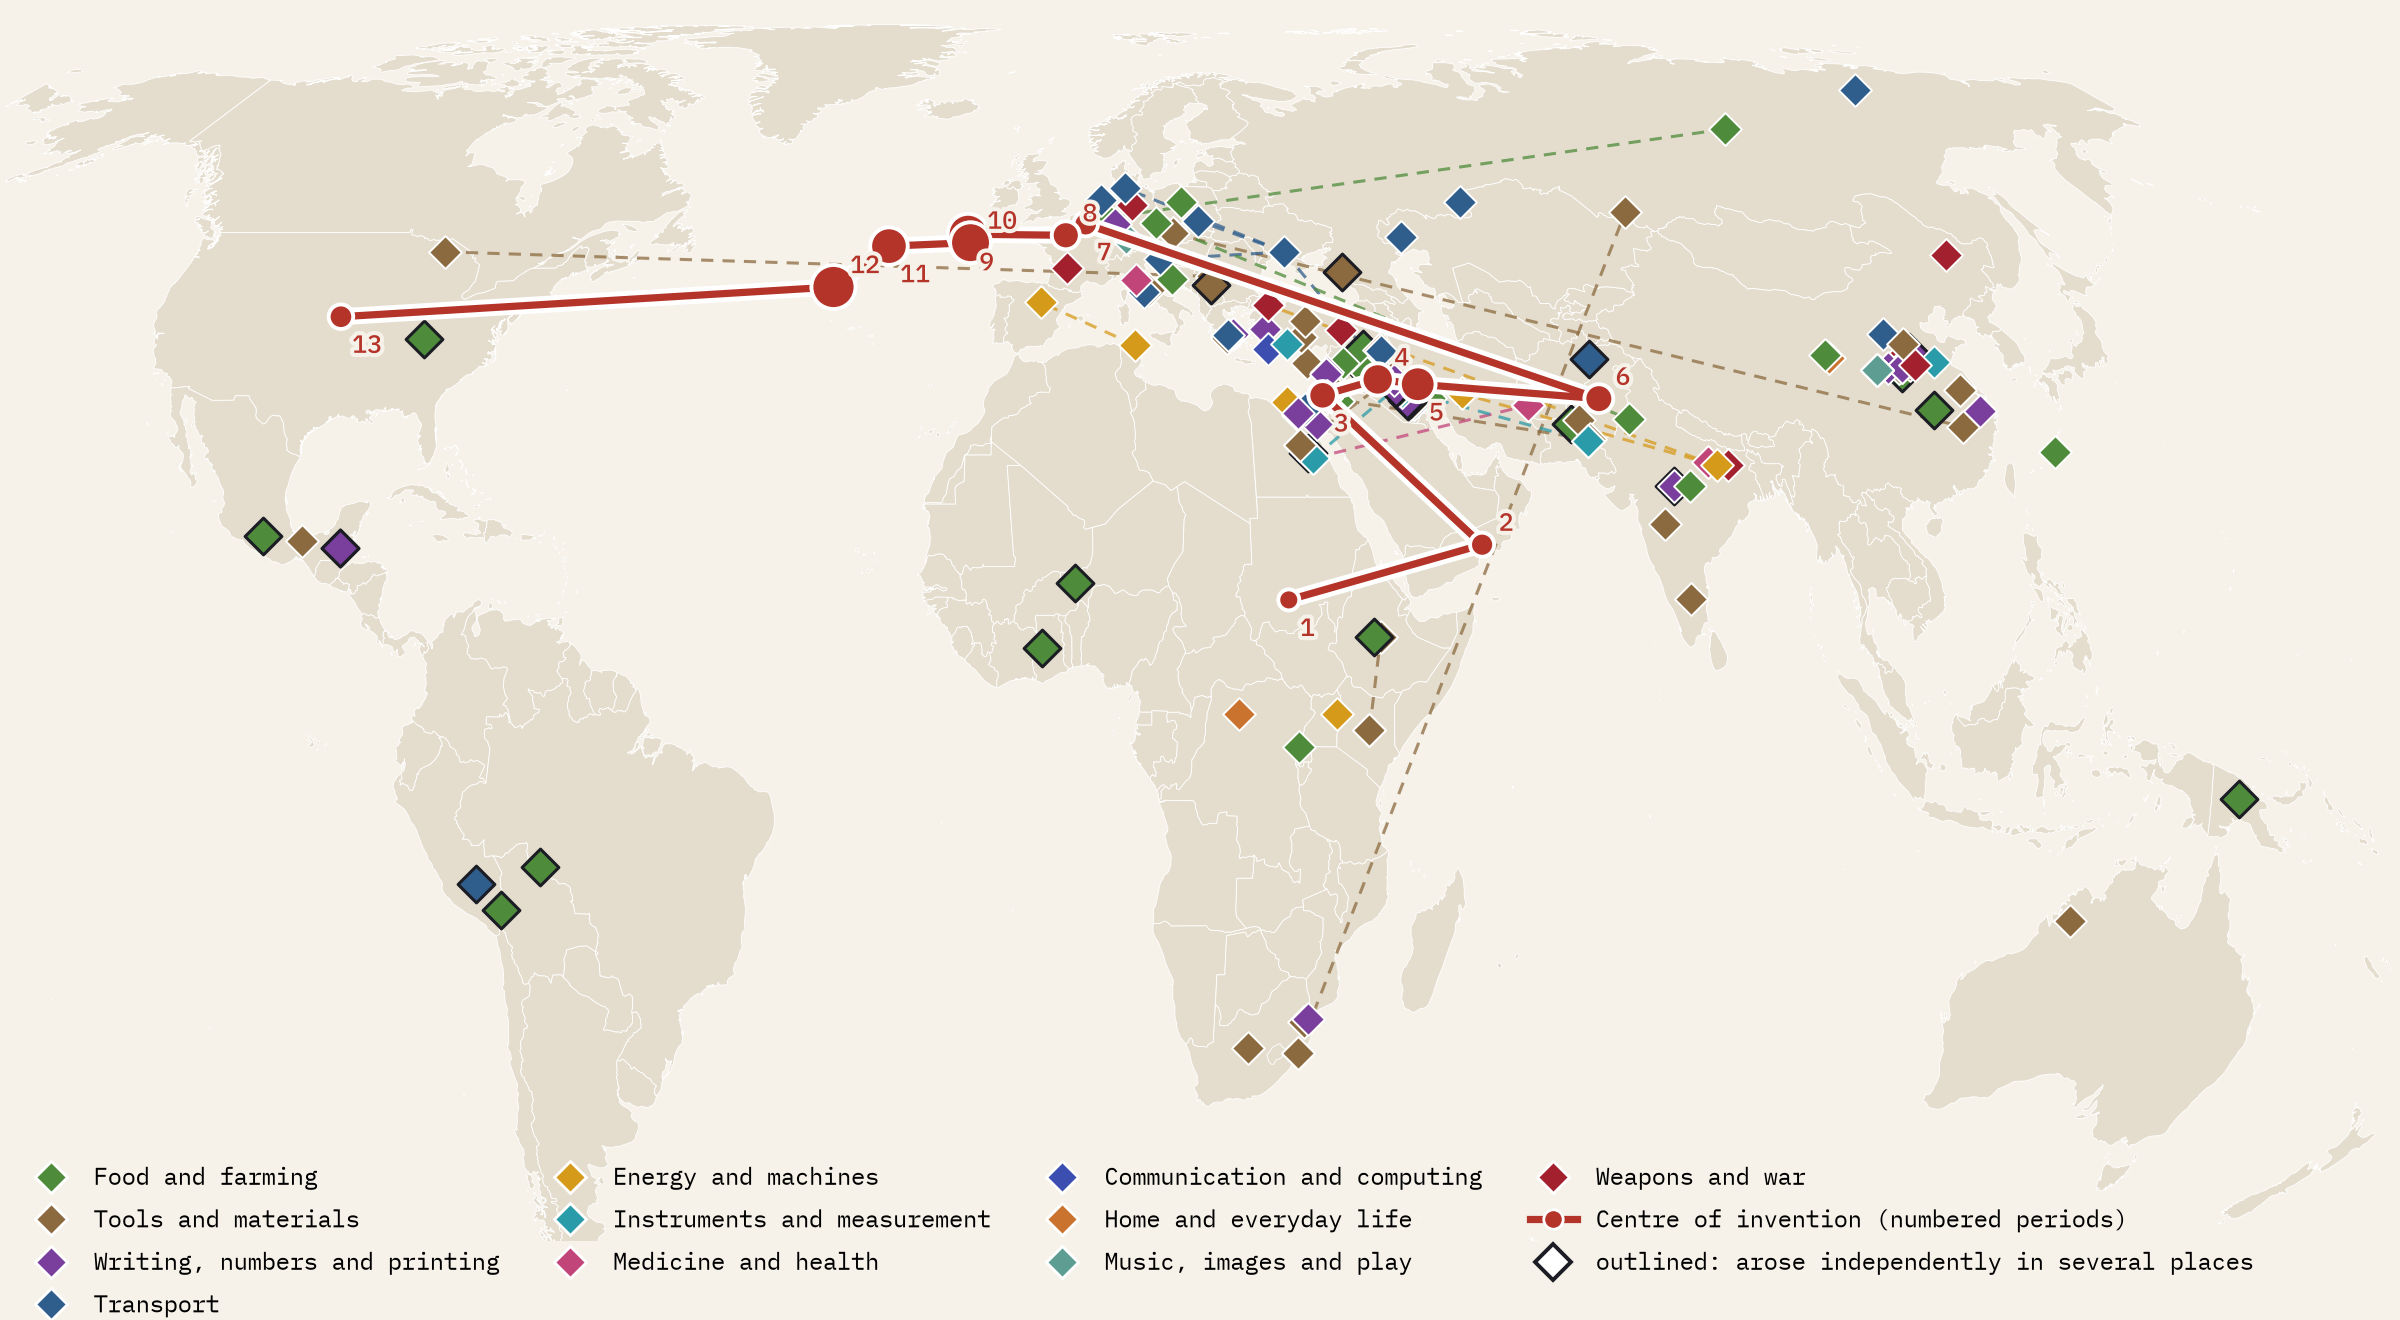
\includegraphics[width=\textwidth]{f_early_map.png}
\caption{The 155 places of 115 early innovations, coloured by kind; outlined diamonds arose independently in several places, dotted lines join early finds or candidate places. Red: the centre of invention of the landmark list, numbered by period as in Table~\ref{tab:centre}. Equal Earth projection.}\label{fig:early}\end{figure}

\begin{table}[tbp]\centering\small\caption{Innovations that arose independently in several places, according to the pages.}\label{tab:indep}\begin{tabular}{p{2.6cm}rp{10.6cm}}\toprule Innovation & Places & Where\\\midrule
Farming & 11 & Fertile Crescent (wheat, barley, lentils); Yangtze basin, China (rice); Yellow River basin, China (millet); Kuk Swamp, New Guinea Highlands (taro, bananas); Southern Mexico (maize, squash, beans); Southwestern Amazon basin (cassava); Lake Titicaca, Andes (potatoes); Ethiopian highlands (coffee, teff, ensete); Sahel (sorghum, pearl millet); West Africa (African rice, yams, oil palm); Eastern North America (sunflower, sumpweed, goosefoot)\\
Livestock & 3 & Fertile Crescent (goats, sheep, pigs, taurine cattle); Baluchistan, Pakistan (humped zebu cattle); East Asia (pigs)\\
Bronze & 3 & Pločnik, Serbia (tin bronze foil, dating disputed); Maykop culture, North Caucasus (arsenical bronze); Sumer, Mesopotamia\\
Writing & 4 & Uruk, Mesopotamia (cuneiform); Abydos, Egypt (hieroglyphs); Late Shang China (oracle bone script); Maya region, Mesoamerica (Maya script)\\
Zero & 3 & Babylon; Maya region, Mesoamerica; India (Brahmagupta)\\
Suspension bridge & 2 & Pre-Columbian South America; Hindu Kush (Afghanistan and Pakistan)\\
\bottomrule\end{tabular}\end{table}

\subsection{The moving centre of invention}
Table~\ref{tab:centre} and Figure~\ref{fig:shares} show where each period's landmarks came from. In the two oldest periods the largest share is sub-Saharan Africa. From 10,000 BC to AD 1, West Asia and North Africa lead: 44\% of the landmarks of 10,000 to 5000 BC, 51\% of those of 5000 to 2000 BC. From AD 1 to 1500, East Asia, in practice China, has 50\% of 26 landmarks: paper, woodblock printing, porcelain, the banknote, gunpowder, movable type. The page lists only a handful of medieval European inventions before Gutenberg, which is itself a choice of the page.

From 1500 to 1700 every landmark on the list is European, and Europe holds 79\% from 1800 to 1850 and 77\% from 1850 to 1900, with North America at 21\% in the latter. North America first leads from 1950 to 2000 (55\%), and all 16 entries since 2000 are American. East Asia's return is modest on this list: 12\% from 1950 to 2000. The Wikidata series agrees: 96\% European from 1800 to 1850, and North America ahead from 1950 to 2000 (45\% against Europe's 40\%). The centre therefore travels from East Africa through the Levant, Mesopotamia and Iran towards South Asia, jumps to northern France, and drifts west across the Atlantic to the United States.

\begin{table}[tbp]\centering\small\caption{The centre of invention: mean latitude and longitude of each period's landmark inventions, and the region with the largest share.}\label{tab:centre}\setlength{\tabcolsep}{4pt}\begin{tabular}{rlrlp{3.3cm}p{3.9cm}}\toprule & Period & Items & Lat, lon & Centre falls & Largest share\\\midrule
1 & 3.3 million to 100,000 years ago & 9 & 12.4, 28.4 & Sudan & Sub-Saharan Africa (67\%)\\
2 & 100,000 to 12,000 years ago & 15 & 17.5, 52.8 & Oman & Sub-Saharan Africa (33\%)\\
3 & 10,000 to 5000 BC & 25 & 31.8, 34.7 & Israel & West Asia and North Africa (44\%)\\
4 & 5000 to 2000 BC & 35 & 33.4, 42.2 & Iraq & West Asia and North Africa (51\%)\\
5 & 2000 BC to AD 1 & 45 & 32.9, 47.4 & Iran & West Asia and North Africa (41\%)\\
6 & AD 1 to 1500 & 26 & 31.5, 70.9 & Pakistan & East Asia (50\%)\\
7 & 1500 to 1700 & 16 & 50.0, 4.0 & France & Europe (100\%)\\
8 & 1700s & 24 & 48.7, 1.0 & France & Europe (92\%)\\
9 & 1800 to 1850 & 62 & 48.8, -13.3 & open sea, nearest land Ireland & Europe (79\%)\\
10 & 1850 to 1900 & 62 & 47.8, -12.8 & open sea, nearest land Ireland & Europe (77\%)\\
11 & 1900 to 1950 & 51 & 47.4, -24.6 & open sea, nearest land Portugal & Europe (63\%)\\
12 & 1950 to 2000 & 74 & 43.0, -31.6 & open sea, nearest land Portugal & North America (55\%)\\
13 & 2000 to 2026 & 16 & 39.8, -98.6 & United States & North America (100\%)\\
\bottomrule\end{tabular}\end{table}

\begin{figure}[tbp]\centering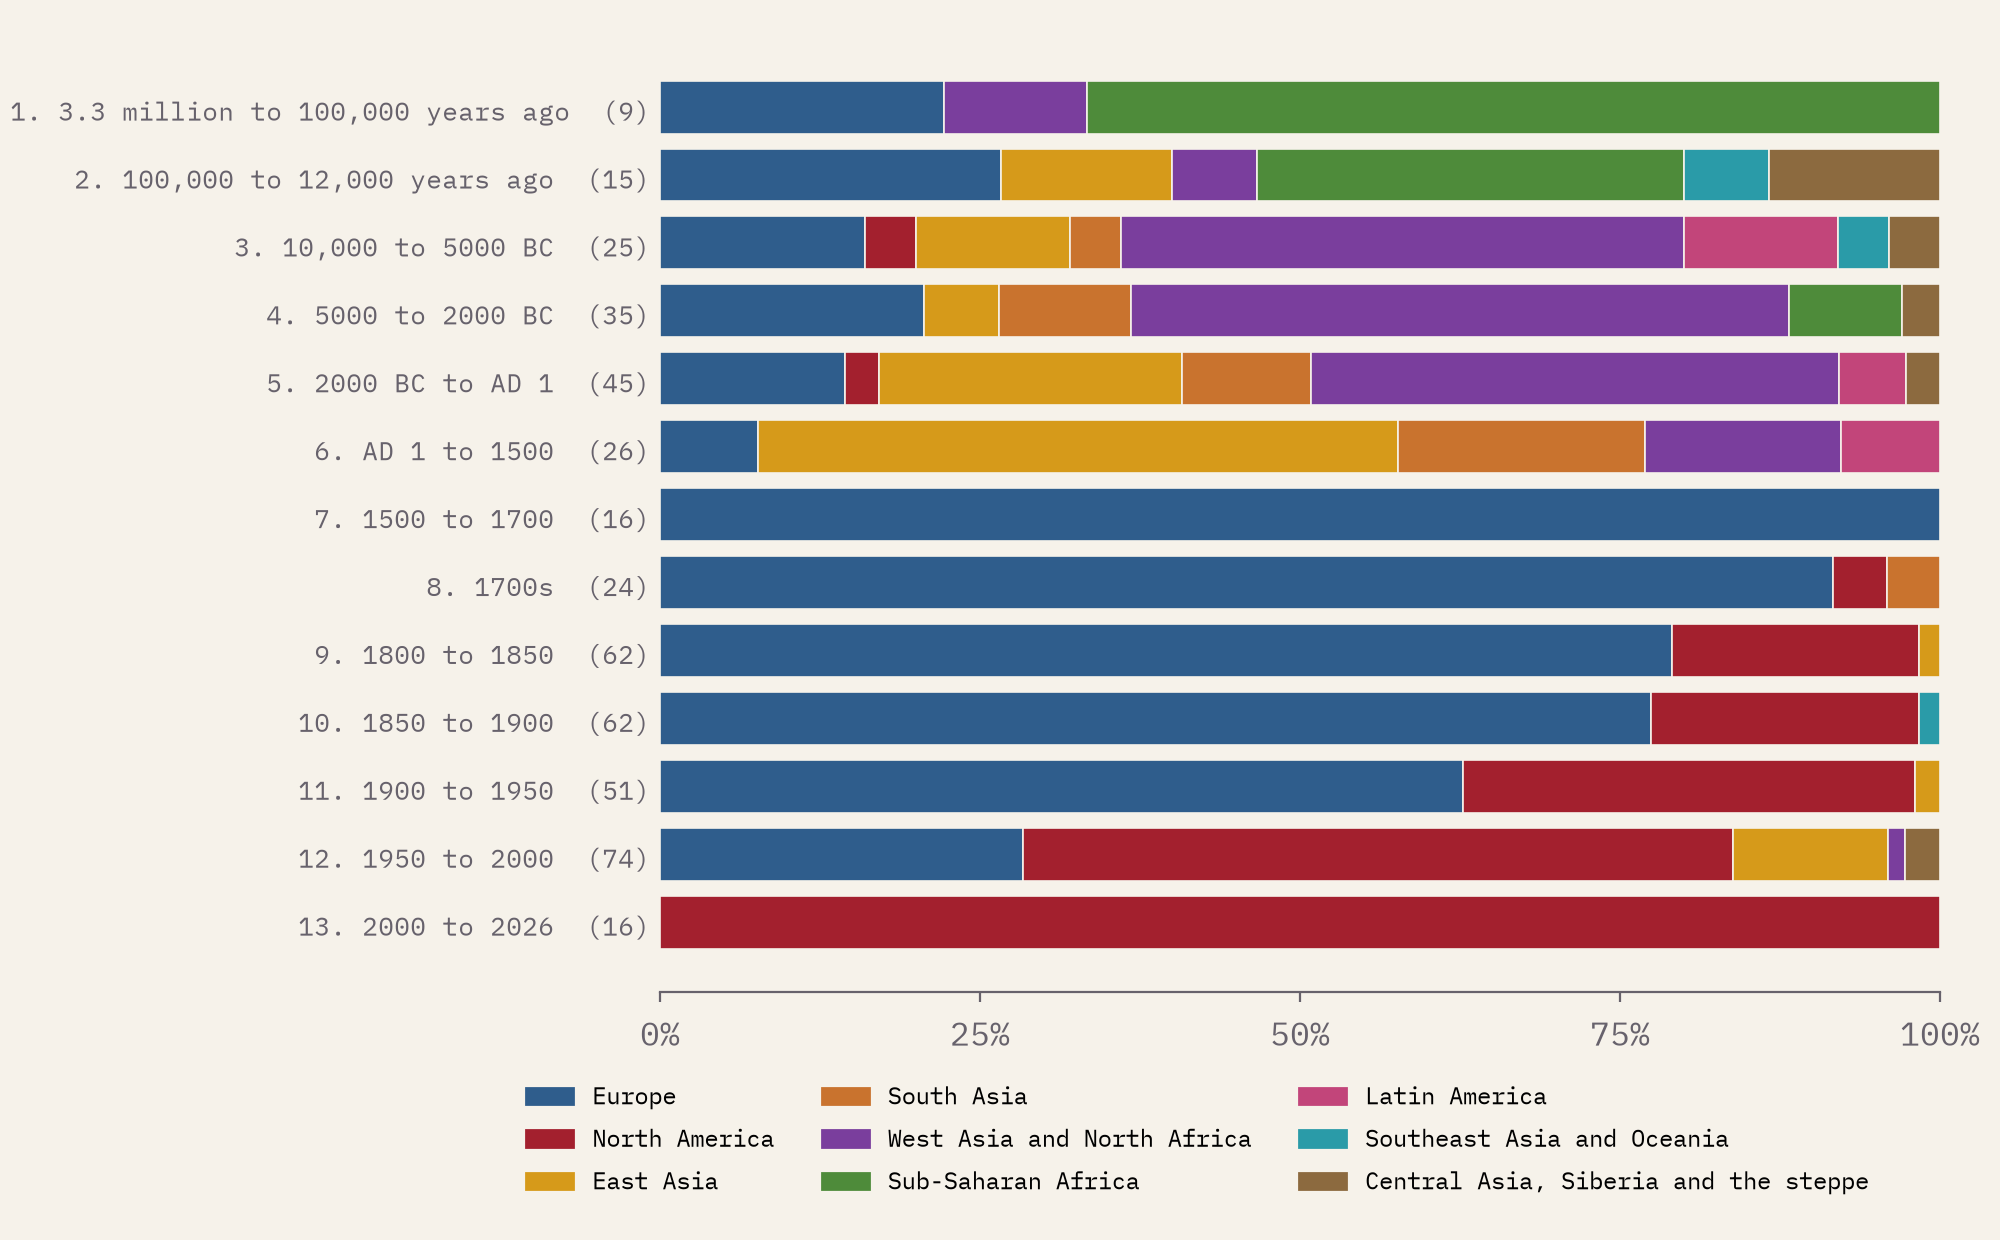
\includegraphics[width=.92\textwidth]{f_shares.png}
\caption{Share of each period's landmark inventions by world region (hand table before 1500, Wikipedia timeline from 1500; number of items in brackets).}\label{fig:shares}\end{figure}

\subsection{Inventions per century}
Both lists accelerate sharply (Figure~\ref{fig:cent}). Wikidata has 177 dated inventions from the nineteenth century and 282 from the twentieth, but 34 from before 1500, and 84\% of its dated inventions are from 1800 or later. Part of this is the real acceleration of invention; part is that recent inventions are documented, patented and attached to named people.

\begin{figure}[tbp]\centering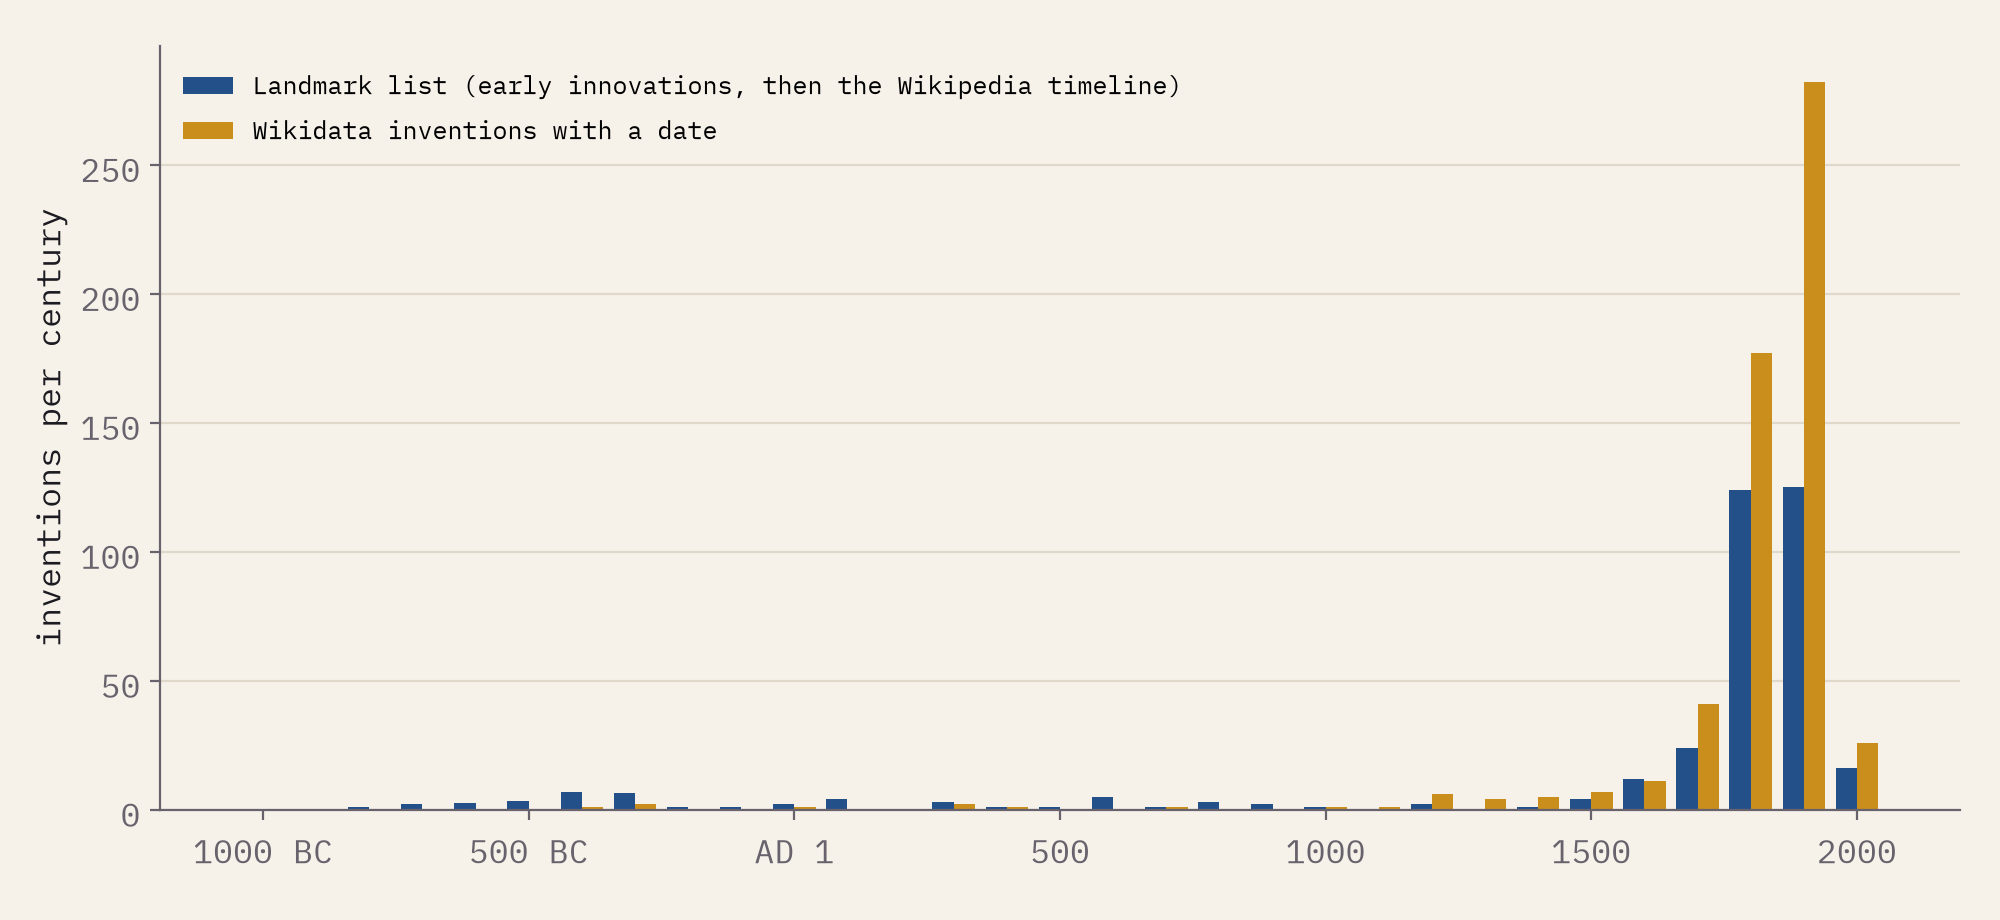
\includegraphics[width=.92\textwidth]{f_centuries.png}
\caption{Inventions per century, 1000 BC to the present: landmark list and dated Wikidata inventions. The last bar is 2000 to 2026.}\label{fig:cent}\end{figure}

\subsection{The Wikidata layer and the most inventive cities}
Of the 1,443 Wikidata inventions, 1,021 (71\%) can be placed and 578 (40\%) have a date (Figure~\ref{fig:wd}). By country the United States leads (260), then the United Kingdom (156), France (122) and Germany (120). By city area London leads with 47, then New York (37), Paris (27) and Vienna (16) (Table~\ref{tab:cities}); most are inventors' birthplaces.

\begin{figure}[tbp]\centering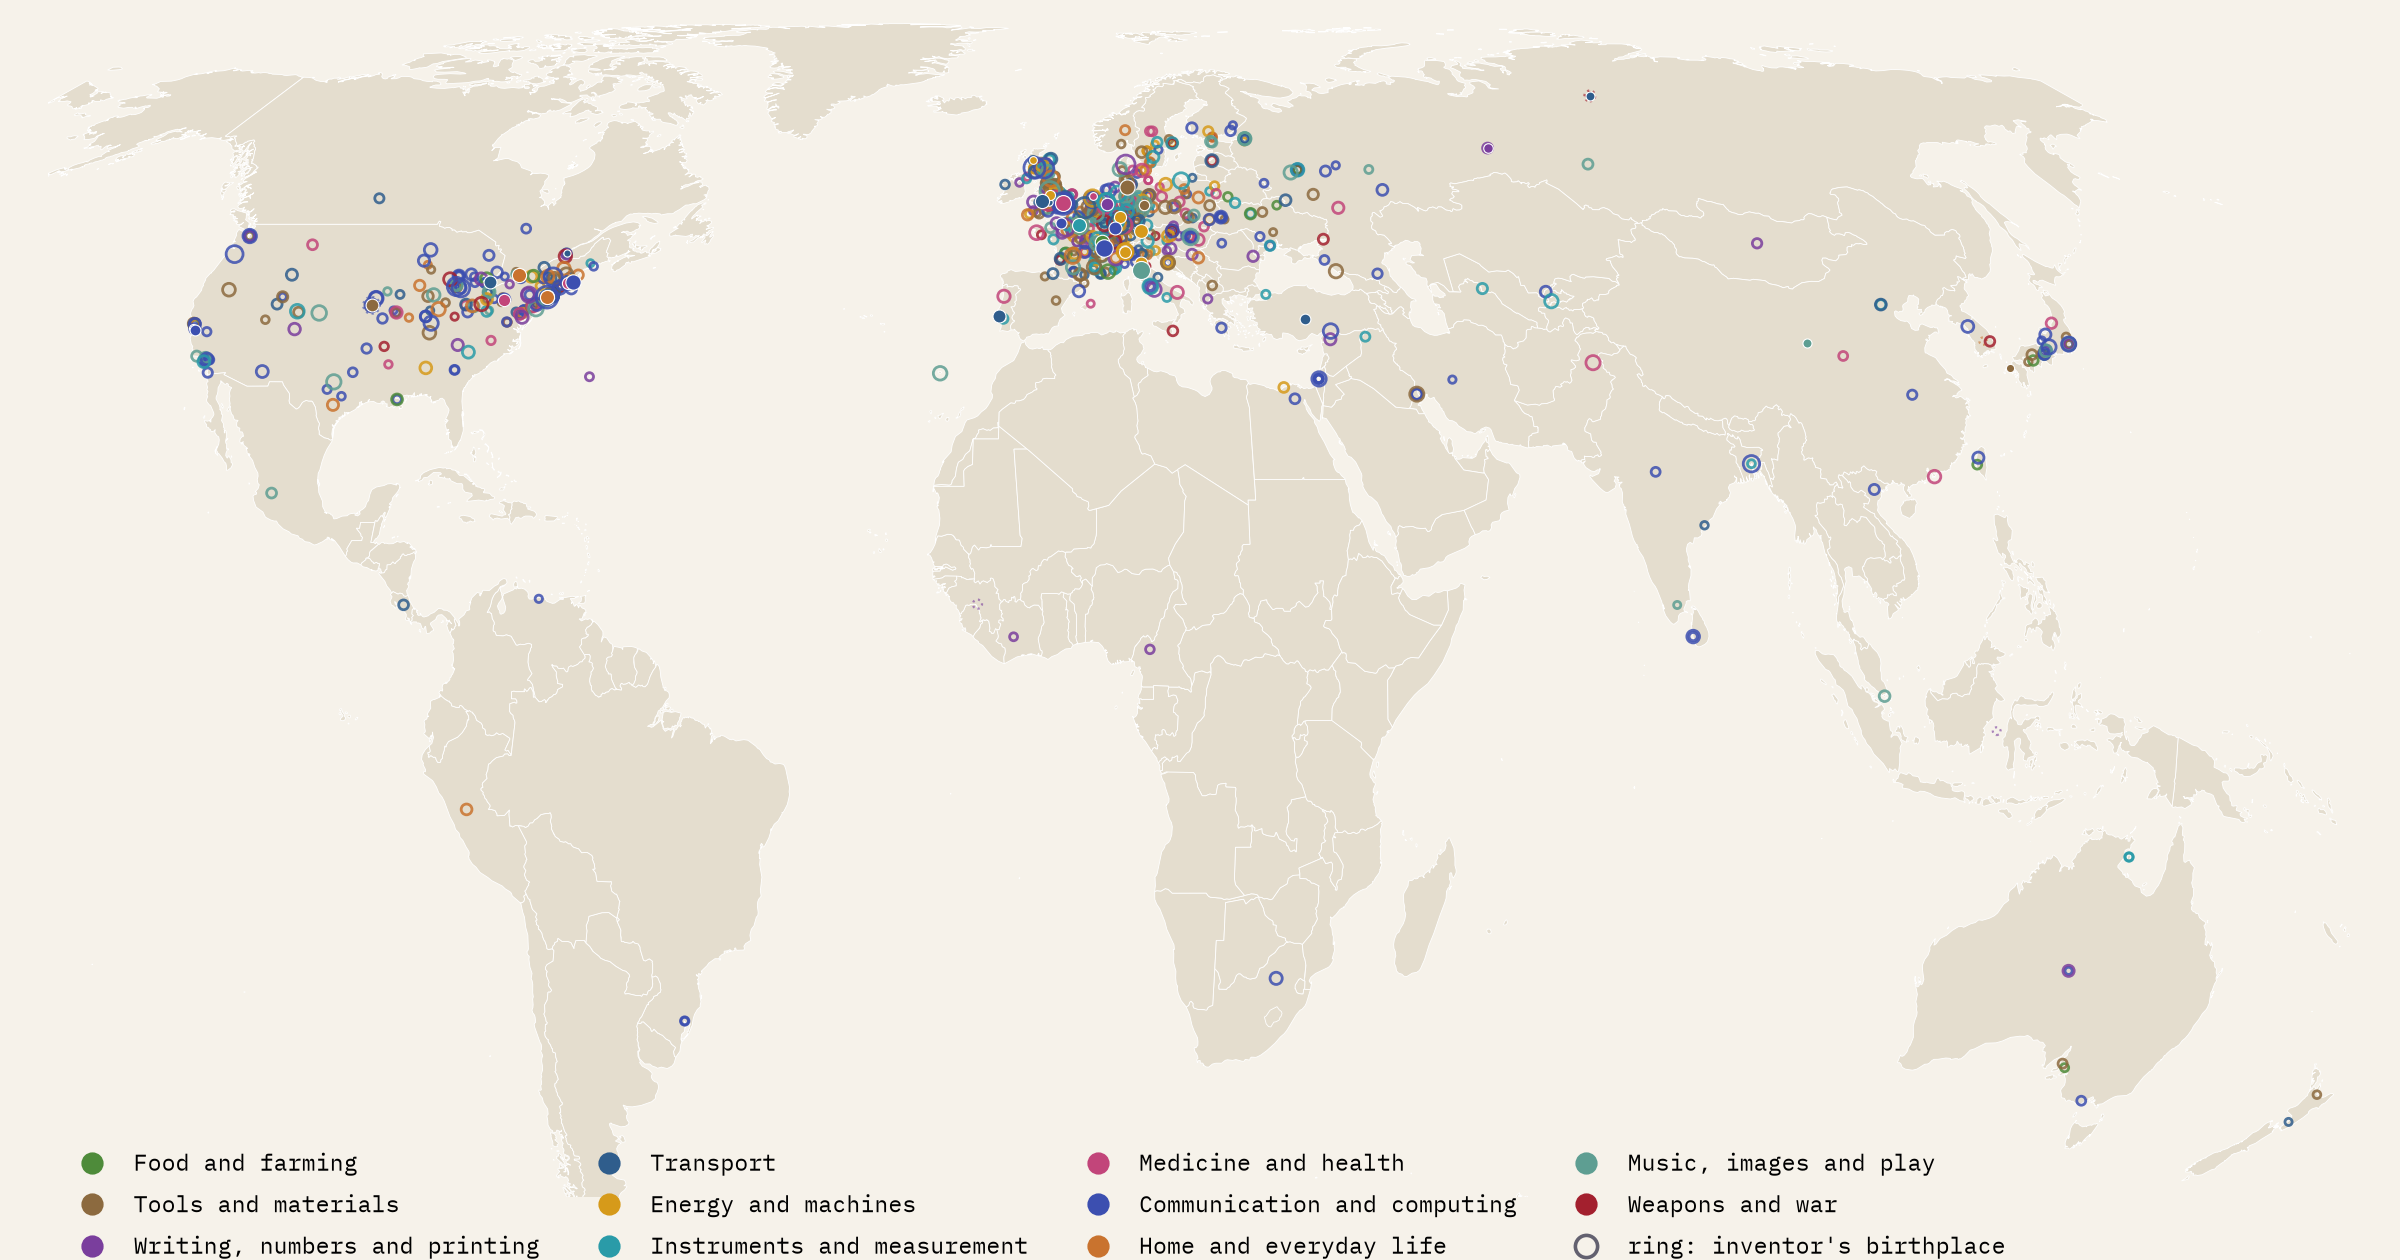
\includegraphics[width=\textwidth]{f_wikidata_map.png}
\caption{Wikidata inventions with 5 or more sitelinks that can be placed (1,021), sized by sitelinks and coloured by kind; filled where Wikidata gives a place of invention, rings where the point is the inventor's birthplace.}\label{fig:wd}\end{figure}

\begin{table}[tbp]\centering\small\caption{City areas with the most Wikidata inventions: all, inventor born there, made or discovered there, and the best known.}\label{tab:cities}\setlength{\tabcolsep}{4pt}\begin{tabular}{llrrrp{6cm}}\toprule City & Country & All & Born & Made & Best known\\\midrule
London & United Kingdom & 47 & 39 & 8 & computer, HTML, web browser\\
New York & United States & 37 & 32 & 5 & Internet, escalator, Ethernet\\
Paris & France & 27 & 23 & 4 & animation, internal combustion engine, sonar\\
Vienna & Austria & 16 & 16 & 0 & triode, Glock, Glock 17\\
Chicago & United States & 12 & 12 & 0 & mobile phone, Hammond organ, WD-40\\
Boston & United States & 10 & 9 & 1 & Morse code, lightning rod, bolometer\\
Edinburgh & United Kingdom & 9 & 9 & 0 & telephone, cloud chamber, Rankine cycle\\
Tokyo & Japan & 8 & 8 & 0 & QR code, karaoke, marker pen\\
Munich & Germany & 8 & 7 & 1 & diesel engine, variometer, Volksempfänger\\
Philadelphia & United States & 8 & 8 & 0 & Internet Message Access Protocol, iron lung, LM317\\
The Hague & Netherlands & 7 & 7 & 0 & capacitor, compact disc, Bluetooth\\
Luton & United Kingdom & 7 & 7 & 0 & Linear B, Bessemer process, octant\\
Berlin & Germany & 7 & 7 & 0 & thermite, breadth-first search, Feistel cipher\\
St. Petersburg & Russia & 7 & 7 & 0 & stop-motion, theremin, drogue parachute\\
San Francisco & United States & 7 & 7 & 0 & Network Time Protocol, jackhammer, hash tree\\
\bottomrule\end{tabular}\end{table}

\subsection{Who gets the credit}
Figure~\ref{fig:bias} sets each region's share of mapped inventions against its share of today's people. Europe and North America hold 91\% of the Wikidata inventions and 95\% of the timeline since 1500, but 14\% of the population; South Asia has 0.8\% of Wikidata's inventions and 24\% of the people, sub-Saharan Africa 0.4\% and 14\%. 83\% of the Wikidata inventions have a named inventor; the hand table, by contrast, names almost no one. Individual credit throws up oddities: Wikidata's only inventor of the car is Ferdinand Verbiest, who built a small steam vehicle in China, and it credits gunpowder to Berthold Schwarz, a legendary German monk, while the Wikipedia timeline dates it to ninth-century China.

\begin{figure}[tbp]\centering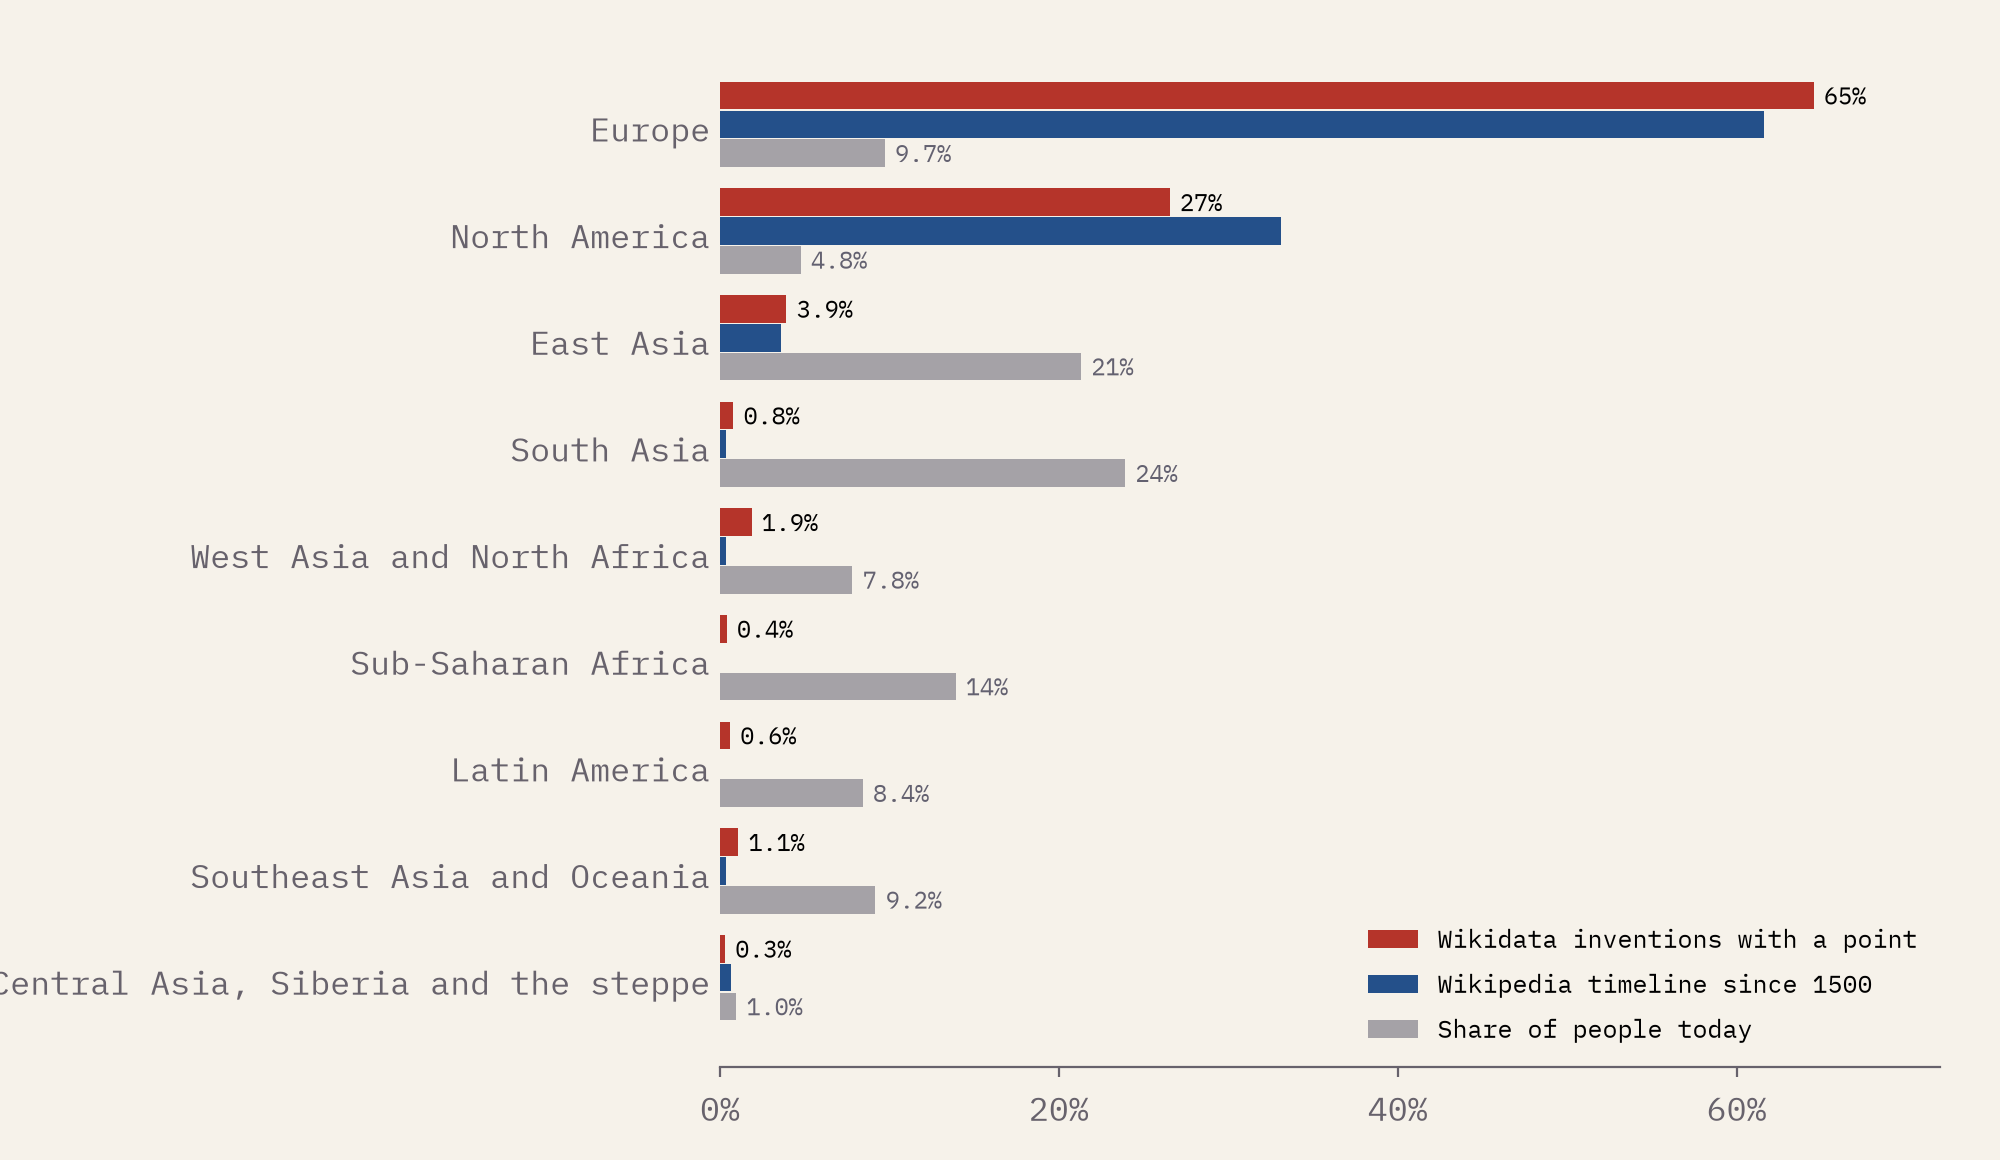
\includegraphics[width=.92\textwidth]{f_bias.png}
\caption{Share of mapped inventions (Wikidata; Wikipedia timeline since 1500) and of present-day population, by region.}\label{fig:bias}\end{figure}

\begin{figure}[tbp]\centering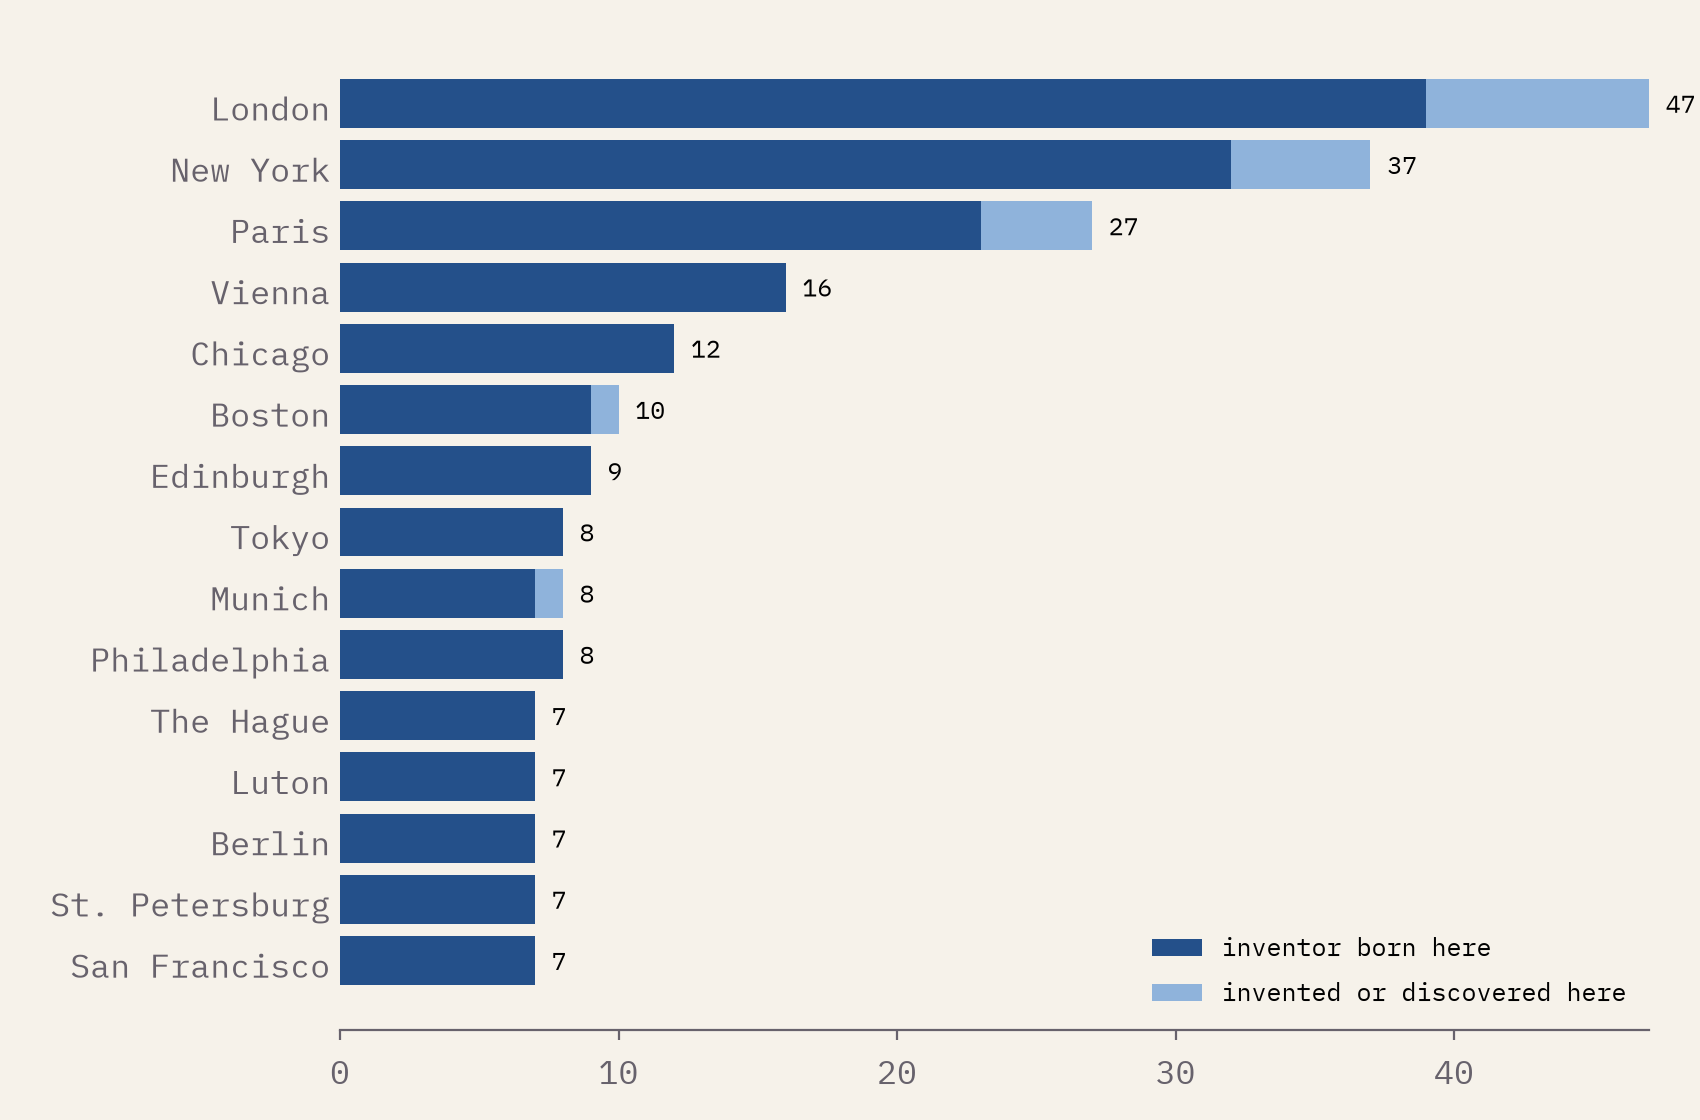
\includegraphics[width=.75\textwidth]{f_cities.png}
\caption{City areas with the most Wikidata inventions, split into inventors born there and inventions made or discovered there.}\label{fig:cities}\end{figure}

\section{Discussion}
Two stories sit in the same map. One is the familiar history of technology: an early world of many independent beginnings, a long period in which West Asia and then China led, and a modern period in which Europe, then North America, took over. The landmark list, curated and short as it is, reproduces that arc clearly, and the much larger Wikidata layer agrees for the modern period.

The other story is about the record. The early innovations were made by peoples, and the pages that describe them hedge, list alternatives and give ranges; the modern entries are attributed to individuals with patents and birthplaces. When the record switches from archaeology to biography, the map switches with it, and the regions whose inventors were not written up in English, or whose innovations were collective, fade. A map of where invention was recorded in English is not the same as a map of where people invented.

\section{Limitations}
The hand table is my reading of nine pages; other pages, and the specialist literature behind them, would add and move rows, and its coordinates are rough by design. The timeline is a curated list whose selection is itself a judgement, and about two in five of its modern entries were placed by hand at country level. The Wikidata filter is imperfect in both directions, especially among items with few sitelinks, and its dates are sparse. The inventor rule places many inventions at birthplaces, which can be far from where the work was done, and picks one inventor when there are several. Shares by period rest on small numbers before 1500. Population is today's and is only a rough yardstick for the past. Present-day borders are used throughout.

\section{Conclusion}
Put back where they came from, the world's inventions trace a centre that moves from East Africa to West Asia, China, Europe and North America, after a beginning in which farming, writing and zero were each invented more than once. The open record of that history is far more European and American than history itself, and far more attached to individual names. Both facts are worth seeing on one map.

\section*{Data and code availability}
All data, code and figures are at \url{https://github.com/Tristan-Hotham/inventions-map} and archived at https://doi.org/10.5281/zenodo.23856736. The interactive atlas is at \url{https://maps.tristanhotham.com/inventions-map/}. The two tables built from Wikipedia text (early innovations and the timeline since 1500) are CC BY-SA 4.0; the other derived data, text and figures are CC BY 4.0, and the code is MIT.

\section*{AI statement}
I wrote the text, with drafting and editing assistance from Claude (Anthropic), which also helped prepare the analysis code. I reviewed and checked all text and results.

\clearpage\section*{Appendix: the early innovations}\footnotesize Sources: TH Timeline of historic inventions; TP Timeline of prehistory; NR Neolithic Revolution; DO Domestication; HW History of writing; WH Wheel; BA Bronze Age; IN List of Indian inventions and discoveries; IG Islamic Golden Age. The quoted passage for every row is in \texttt{data/early\_innovations.csv}.
\setlength{\tabcolsep}{4pt}\begin{longtable}{p{3.3cm}p{5.2cm}p{3.3cm}p{1.7cm}l}\caption{Early innovations, places and dates as the pages give them.}\label{tab:early}\\\toprule Innovation & Place & Date & Kind & Page\\\midrule\endhead
Stone tools & Kenya & 3.3 million years ago to 2.6 million years ago & finds & TH\\
Stone tools & Ethiopia (Oldowan tools) & 3.3 million years ago to 2.6 million years ago & finds & TH\\
Hand axes (Acheulean stone tools) & Kenya & 1.8 million years ago & single & TH\\
Control of fire & Africa (the page names Homo erectus but no place) & 1.5 million years ago & single & TH\\
Cooking & Middle East & 1,000,000 years ago to 778,000 years ago & single & TH\\
Hafting (fixing a stone point to a handle) & South Africa & 498,000 years ago & single & TH\\
Wooden spears & Schöningen, Germany & 335,000 years ago to 298,000 years ago & single & TH\\
Glue (birch tar) & Central Italy & 198,000 years ago & single & TH\\
Clothing & Africa (continent only) & 168,000 years ago to 88,000 years ago & single & TH\\
Harpoons & Democratic Republic of the Congo & 88,000 years ago & single & TH\\
Bow and arrow & Sibudu Cave, South Africa & 68,000 years ago to 58,000 years ago & single & TH\\
Sewing needle & Sibudu Cave, South Africa & 68,000 years ago to 58,000 years ago & finds & TH\\
Sewing needle & Denisova Cave, Altai, Siberia & 48,000 years ago & finds & TP\\
Ground stone axe & Australia & 47,000 years ago to 43,000 years ago & single & TH\\
Mining (for red ochre) & Eswatini & 45,000 years ago & single & TH\\
Tally sticks (Lebombo bone) & Eswatini & 42,000 years ago to 40,000 years ago & single & TH\\
Flute & Germany & 40,000 years ago & single & TH\\
Fired clay & Dolní Věstonice, Czech Republic (figurines) & 26,000 years ago to 22,000 years ago & finds & TP\\
Fired clay & Xianren Cave, China (pottery vessels) & 18050 BC to 17050 BC & finds & TP\\
Spear-thrower (atlatl) & France & 15550 BC & single & TH\\
Domestication of the dog & Siberia & 21,000 years ago & finds & TH\\
Domestication of the dog & Bonn-Oberkassel, Germany (oldest agreed remains) & 12250 BC & finds & TP\\
Fish hook & Okinawa, Japan & 20,000 years ago & single & TH\\
Bread & Jordan & 12550 BC & single & TH\\
Spindle whorl & Nahal Ein Gev II, Israel & 10050 BC & single & TH\\
Farming & Fertile Crescent (wheat, barley, lentils) & 10000 BC to 8000 BC & independent & NR\\
Farming & Yangtze basin, China (rice) & 11550 BC to 6250 BC & independent & NR\\
Farming & Yellow River basin, China (millet) & 6050 BC to 5550 BC & independent & NR\\
Farming & Kuk Swamp, New Guinea Highlands (taro, bananas) & 8000 BC to 7000 BC & independent & NR\\
Farming & Southern Mexico (maize, squash, beans) & 7000 BC to 6000 BC & independent & NR\\
Farming & Southwestern Amazon basin (cassava) & 8900 BC to 8300 BC & independent & TP\\
Farming & Lake Titicaca, Andes (potatoes) & 8000 BC to 5000 BC & independent & TH\\
Farming & Ethiopian highlands (coffee, teff, ensete) & 3050 BC to 2050 BC & independent & NR\\
Farming & Sahel (sorghum, pearl millet) & 3050 BC to 2050 BC & independent & NR\\
Farming & West Africa (African rice, yams, oil palm) & 3050 BC to 2050 BC & independent & NR\\
Farming & Eastern North America (sunflower, sumpweed, goosefoot) & 2500 BC to 1050 BC & independent & NR\\
Livestock (goats, sheep, pigs, cattle) & Fertile Crescent (goats, sheep, pigs, taurine cattle) & 9050 BC to 8050 BC & independent & DO\\
Livestock (goats, sheep, pigs, cattle) & Baluchistan, Pakistan (humped zebu cattle) & 7050 BC to 6050 BC & independent & DO\\
Livestock (goats, sheep, pigs, cattle) & East Asia (pigs) & 6050 BC & independent & DO\\
Domestication of the cat & Fertile Crescent & 8050 BC & single & DO\\
Alcohol fermentation (mead) & Southwest Asia & 10000 BC to 9000 BC & single & TH\\
Mudbricks & Jericho & 9000 BC & single & TH\\
Water well & Cyprus & 8400 BC & single & TH\\
Boat (dugout canoe) & Pesse, Netherlands & 8040 BC to 7510 BC & single & TH\\
Dog sled & Siberia & 7000 BC & single & TH\\
Copper working & Great Lakes, North America (Old Copper Complex tools) & 7500 BC to 6500 BC & finds & TH\\
Copper working & Pločnik and Belovode, Serbia (copper smelting) & 5500 BC & finds & TP\\
Lead smelting & Çatalhöyük, Turkey & 6500 BC & single & TH\\
Kiln & Mesopotamia & 6000 BC & single & TH\\
Irrigation & Khuzistan, Iran & 6000 BC to 5001 BC & single & TH\\
Cheese & Poland & 5500 BC to 5200 BC & finds & TH\\
Cheese & Dalmatian coast, Croatia & 5500 BC to 5200 BC & finds & TH\\
Sailing & Mesopotamia & 5500 BC & single & TH\\
Cotton thread & Mehrgarh, Indus Valley & 5000 BC & single & TH\\
Lost-wax casting & Palestine & 4500 BC to 3500 BC & candidates & TH\\
Lost-wax casting & Indus Valley & 4500 BC to 3500 BC & candidates & TH\\
Paved roads & Ur, Mesopotamia & 4000 BC & single & TH\\
Plumbing (clay pipes) & Nippur, Mesopotamia & 4000 BC & single & TH\\
Lock & Nineveh, Assyria & 4000 BC & single & TH\\
Wheel and wagon & North of the Black Sea (miniature clay wheels) & 4100 BC to 4000 BC & finds & WH\\
Wheel and wagon & Uruk, Mesopotamia (wagon pictographs) & 3500 BC to 3350 BC & finds & WH\\
Wheel and wagon & Bronocice, Poland (wagon on a pot) & 3631 BC to 3380 BC & finds & WH\\
Wheel and wagon & Northern Germany (wheel ruts) & 3400 BC & finds & WH\\
Wheel and wagon & Ljubljana Marshes, Slovenia (oldest wooden wheel) & 3130 BC & finds & WH\\
Potter's wheel & Ur, Mesopotamia & 4000 BC to 3100 BC & single & WH\\
Spoked wheel and chariot & Sintashta culture, southern Urals & 2000 BC & single & WH\\
Domestication of the horse & Eurasian steppes & 3500 BC & single & TH\\
Silk & China & 3630 BC & single & TH\\
Plough & Bubeneč, Czech Republic & 3500 BC & finds & TH\\
Plough & Kalibangan, Indus Valley & 2800 BC & finds & TH\\
Bronze & Pločnik, Serbia (tin bronze foil, dating disputed) & 4650 BC & independent & BA\\
Bronze & Maykop culture, North Caucasus (arsenical bronze) & 3600 BC to 3400 BC & independent & BA\\
Bronze & Sumer, Mesopotamia & 3600 BC to 3400 BC & independent & BA\\
Writing & Uruk, Mesopotamia (cuneiform) & 3400 BC to 3100 BC & independent & HW\\
Writing & Abydos, Egypt (hieroglyphs) & 3400 BC to 3100 BC & independent & HW\\
Writing & Late Shang China (oracle bone script) & 1250 BC to 1050 BC & independent & HW\\
Writing & Maya region, Mesoamerica (Maya script) & 300 BC to 200 BC & independent & HW\\
Sword & Arslantepe, Turkey & 3300 BC & single & TH\\
Papyrus & Egypt & 3000 BC to 2560 BC & single & TH\\
Dice & Burnt City, Iran & 2800 BC to 2500 BC & single & TH\\
Prosthesis & Ancient Egypt & 3000 BC to 2800 BC & finds & TH\\
Prosthesis & Iran (artificial eye) & 3000 BC to 2800 BC & finds & TH\\
Rhinoplasty & Egypt & 3000 BC to 2500 BC & single & TH\\
Ruler (measuring rod) & Nippur, Mesopotamia & 2650 BC & single & TH\\
Public sewers and sanitation & Mohenjo-daro, Indus Valley & 2600 BC & single & TH\\
Balance weights and scales & Egypt (Fourth Dynasty) & 2600 BC & single & TH\\
Fork & Qijia culture, China & 2400 BC & single & TH\\
Iron smelting & Kaman-Kalehöyük, Turkey & 2200 BC to 2000 BC & single & TH\\
Water clock & Babylonia & 2000 BC to 1600 BC & candidates & TH\\
Water clock & Mohenjo-daro, Indus Valley & 2000 BC & candidates & TH\\
Scissors & Mesopotamia & 2000 BC & single & TH\\
Noodles & Lajia, China & 2000 BC & single & TH\\
Alphabet (Proto-Sinaitic script) & Sinai, Egypt & 1850 BC to 1800 BC & single & HW\\
Phoenician alphabet & Phoenicia (Lebanon) & 1050 BC & single & HW\\
Greek alphabet, the first with vowels & Greece & 800 BC & single & HW\\
Sundial & Ancient Egypt & 1500 BC & candidates & TH\\
Sundial & Babylonia & 1500 BC & candidates & TH\\
Glass & Mesopotamia & 1500 BC & candidates & TH\\
Glass & Ancient Egypt & 1500 BC & candidates & TH\\
Seed drill & Babylonia & 1500 BC & single & TH\\
Rubber & Mesoamerica (the Mesoamerican ballgame) & 1400 BC & single & TH\\
Concrete & Tiryns, Greece & 1400 BC to 1200 BC & single & TH\\
Distillation & Mesopotamia (Akkadian tablets) & 1200 BC & single & TH\\
Saddle & Assyria & 700 BC & single & TH\\
Crossbow & China & 650 BC & single & TH\\
Coins & Phoenicia (Lebanon) & 600 BC & candidates & TH\\
Coins & Lydia (Sardis, Turkey) & 600 BC & candidates & TH\\
Wagonway (the Diolkos) & Isthmus of Corinth, Greece & 600 BC & single & TH\\
Crank (rotary quern) & Carthage & 550 BC to 500 BC & candidates & TH\\
Crank (rotary quern) & Celtiberian Spain & 500 BC to 400 BC & candidates & TH\\
High-carbon (Wootz) steel & South India & 600 BC to 300 BC & single & TH\\
Systematic surgery (cataract surgery, plastic surgery) & Northern India (Sushruta Samhita) & 600 BC to 200 BC & single & TH\\
Cast iron & Luhe County, Jiangsu, China & 500 BC to 401 BC & single & TH\\
Catapult & Magadha, India & 485 BC & single & TH\\
Camera obscura & China (described by Mozi) & 400 BC & single & TH\\
Zero & Babylon & 400 BC to 300 BC & independent & TH\\
Zero & Maya region, Mesoamerica & AD 1 to AD 300 & independent & TH\\
Zero & India (Brahmagupta) & AD 628 & independent & IN\\
Decimal place-value numerals & Indian subcontinent & AD 1 to AD 600 & single & IN\\
Traction trebuchet & China & 400 BC to 301 BC & single & TH\\
Gears & China & 400 BC to 301 BC & single & TH\\
Nailed horseshoe & Etruria, Italy & 400 BC to 301 BC & single & TH\\
Analogue computer (Antikythera mechanism) & Rhodes, Greece (possibly) & 300 BC to 201 BC & single & TH\\
Archimedes' screw & Nile, Egypt & 300 BC to 201 BC & single & TH\\
Canal lock & Canal of the Pharaohs, Egypt & 283 BC to 246 BC & single & TH\\
Water wheel & India (Pali texts) & 400 BC to 301 BC & candidates & TH\\
Water wheel & Persia & 350 BC & candidates & TH\\
Water wheel & Hellenistic world (Philo of Byzantium) & 280 BC to 220 BC & candidates & TH\\
Blast furnace & China & 300 BC to 101 BC & single & TH\\
Paper & Han dynasty China & 200 BC to AD 200 & single & TH+HW\\
Compass & Han dynasty China & 206 BC & single & TH\\
Astrolabe & Perga (Apollonius of Perga) & 200 BC to 150 BC & single & TH\\
Glass blowing & Jerusalem & 37 BC to 14 BC & single & TH\\
Aeolipile (simple steam turbine) & Alexandria (Hero of Alexandria) & AD 1 to AD 100 & single & TH\\
Seismometer & Han dynasty China (Zhang Heng) & AD 132 & single & TH\\
Woodblock printing & Han dynasty China & AD 100 to AD 220 & single & TH\\
Crystallised sugar & India & AD 1 to AD 300 & single & IN\\
Suspension bridge & Pre-Columbian South America & AD 301 to AD 400 & independent & TH\\
Suspension bridge & Hindu Kush (Afghanistan and Pakistan) & AD 301 to AD 400 & independent & TH\\
Horse collar & Northern and Southern dynasties China & AD 401 to AD 500 & single & TH\\
Spinning wheel (charkha) & Maharashtra, India & AD 500 to 1000 & single & TH\\
Toilet paper & Sui dynasty China & AD 589 & single & TH\\
Toothbrush & Tang dynasty China & AD 619 & single & TH\\
Greek fire & Constantinople & AD 672 & single & TH\\
Banknote & Tang dynasty China & AD 618 to AD 700 & single & TH\\
Porcelain & Northern China & AD 618 to AD 700 & single & TH\\
Gunpowder & Tang dynasty China & AD 801 to AD 900 & single & TH\\
Playing cards & Tang dynasty China & AD 801 to AD 900 & single & TH\\
Algebra (al-Khwarizmi's text) and Indian arithmetic in the Islamic world & Baghdad & AD 825 to AD 830 & single & IG+IN\\
Fire lance (the first firearm) & Song dynasty China & AD 901 to 1000 & single & TH\\
Fountain pen & Fatimid Egypt & AD 974 & single & TH\\
Movable type & Song dynasty China (Bi Sheng) & 1040 to 1088 & single & TH\\
Hand cannon & Heilongjiang, China & 1201 to 1300 & single & TH\\
Eyeglasses & Italy & 1286 & single & TH\\
Printing press with movable type & Mainz, Germany (Johannes Gutenberg) & 1439 & single & TH\\
\bottomrule\end{longtable}\normalsize

\begin{thebibliography}{9}
\bibitem[Bast and Buchhold(2017)]{qlever} Bast, H. and Buchhold, B. (2017) QLever: a query engine for efficient SPARQL+text search. \emph{Proceedings of the 2017 ACM Conference on Information and Knowledge Management}, 647 to 656. \url{https://qlever.cs.uni-freiburg.de/}
\bibitem[Diamond(1997)]{diamond} Diamond, J. (1997) \emph{Guns, Germs, and Steel: The Fates of Human Societies}. New York: W. W. Norton.
\bibitem[Edgerton(2006)]{edgerton} Edgerton, D. (2006) \emph{The Shock of the Old: Technology and Global History since 1900}. London: Profile Books.
\bibitem[Graham et al.(2014)]{graham} Graham, M., Hogan, B., Straumann, R. K. and Medhat, A. (2014) Uneven geographies of user-generated information: patterns of increasing informational poverty. \emph{Annals of the Association of American Geographers}, 104(4), 746 to 764.
\bibitem[Larson et al.(2014)]{larson} Larson, G. et al. (2014) Current perspectives and the future of domestication studies. \emph{Proceedings of the National Academy of Sciences}, 111(17), 6139 to 6146.
\bibitem[Mokyr(1990)]{mokyr} Mokyr, J. (1990) \emph{The Lever of Riches: Technological Creativity and Economic Progress}. New York: Oxford University Press.
\bibitem[Natural Earth(2026)]{naturalearth} Natural Earth (2026) Admin 0 countries and populated places. Public domain. \url{https://www.naturalearthdata.com/}
\bibitem[Needham(1954)]{needham} Needham, J. (1954) \emph{Science and Civilisation in China}, volume 1. Cambridge: Cambridge University Press.
\bibitem[Vrandečić and Krötzsch(2014)]{wikidata} Vrandečić, D. and Krötzsch, M. (2014) Wikidata: a free collaborative knowledgebase. \emph{Communications of the ACM}, 57(10), 78 to 85.
\bibitem[Wikipedia contributors(2026)]{wp} Wikipedia contributors (2026) Timeline of historic inventions; Timeline of prehistory; Neolithic Revolution; Domestication; History of writing; Wheel; Bronze Age; List of Indian inventions and discoveries; Islamic Golden Age. \emph{English Wikipedia}, CC BY-SA 4.0. Revision numbers in the data files. \url{https://en.wikipedia.org/}
\end{thebibliography}
\end{document}
